%% Template for a preprint Letter or Article for submission
%% to the journal Nature.
%% Written by Peter Czoschke, 26 February 2004
%%


\documentclass{nature}
\usepackage{amsmath,amssymb}
\usepackage{hyperref}
\usepackage{cite}
\usepackage{graphicx}
\usepackage[right]{lineno}
%\graphicspath{ {figures/} }
\newcommand*{\bigcdot}{\raisebox{-0.25ex}{\scalebox{1.2}{$\cdot$}}}

%% make sure you have the nature.cls and naturemag.bst files where
%% LaTeX can find them

\bibliographystyle{naturemag}

\title{Neuron's Eye View: Inferring Features of Complex Stimuli from Neural Responses}

%% Notice placement of commas and superscripts and use of &
%% in the author list

\author{Xin (Cindy) Chen$^{1,3}$, Jeffrey M. Beck$^{2, 3}$ \& John M. Pearson$^{1, 3}$}


\begin{document}

\maketitle

\begin{affiliations}
 \item Duke Institute for Brain Sciences, Duke University, Durham, North Carolina, USA
 \item Department of Neurobiology, Duke University Medical Center, Durham, North Carolina, USA
 \item Center for Cognitive Neuroscience, Duke University, Durham, North Carolina, USA
\end{affiliations}

\begin{abstract}
%For Nature, the abstract is really an introductory paragraph set
%in bold type.  This paragraph must be ``fully referenced'' and
%less than 180 words for Letters.  This is the thing that is
%supposed to be aimed at people from other disciplines and is
%arguably the most important part to getting your paper past the
%editors.  End this paragraph with a sentence like ``Here we
%show...'' or something similar.

Experiments that study the neural encoding of stimuli typically require advance knowledge of the relevant features coded by a given population of neurons. For domains as complex as social interaction or natural movement, however, the relevant feature space is poorly understood, and an arbitrary \emph{a priori} choice of features may give rise to confirmation bias. Here we present a Bayesian model for exploratory data analysis that is capable of automatically identifying the features present in unstructured stimuli based solely on neuronal responses. Our approach is unique within the class of latent state space models of neural activity in that it assumes firing rates of neurons are sensitive to multiple discrete time-varying features tied to the \emph{stimulus}, each of which has Markov (or semi-Markov) dynamics. We derive a fast variational Bayesian inference algorithm and show that it correctly recovers hidden features in synthetic data, as well as reproducing key scientific results in a pair of prototypical neural data sets.

\end{abstract}

%Then the body of the main text appears after the intro paragraph.
%Figure environments can be left in place in the document.
%\verb|\includegraphics| commands are ignored since Nature wants
%the figures sent as separate files and the captions are
%automatically moved to the end of the document (they are printed
%out with the \verb|\end{document}| command. However, tables must
%be manually moved to the end of the document, after the addendum.

\linenumbers

\section*{Introduction}
The question of how the brain encodes information from the natural world forms one of the primary areas of study within neuroscience. For many sensory systems, particularly vision and audition, the discovery that single neurons modulate their firing of action potentials in response to particular stimulus features has proven foundational for theories of sensory function. Indeed, neuronal responses to contrast, edges, and motion direction appear to form fundamental primitives on which higher-level visual abstractions are built. Yet many higher-level abstractions like social interaction do not exist in a stimulus space with obvious axes. As a result, experimenters must choose \emph{a priori} features of interest in constructing their stimulus sets, with the result that cells may appear weakly tuned due to misalignment of stimulus and neural axes.

In vision, methods like reverse correlation have proven successful in elucidating response properties of some cell types, but such techniques rely on a well-behaved stimulus space and a highly constrained encoding model in order to achieve sufficient statistical power to perform inference \cite{steveninck1988realtime,ringach2004reverse,ringach2002receptive}. However, natural stimuli are known to violate both criteria, generating patterns of neural activity that differ markedly from those observed in controlled experiments with limited stimulus complexity \cite{ringach2002receptive,sharpee2004analyzing,Vinje2000-dx}. Information-based approaches have gone some way in addressing this challenge \cite{sharpee2004analyzing}, but this approach assumes a metric structure on stimuli in order to perform optimization, and was recently shown to be strongly related to standard Poisson regression models\cite{Williamson2013-rg}.

More recently, Gallant and collaborators have tackled this problem in the context of fMRI, demonstrating that information present in the blood oxygen level-dependent (BOLD) signal is sufficient to classify and map the representation of natural movie stimuli across the brain \cite{Vu2011-da,Huth2012-cj,Stansbury2013-nm}. These studies have used a number of modeling frameworks, from Latent Dirichlet Allocation for categorizing scene contents \cite{Stansbury2013-nm} to regularized linear regression \cite{Huth2012-cj} to sparse nonparametric models \cite{Vu2011-da} in characterizing brain encoding of stimuli, but in each case, models were built on pre-labeled training data. Clearly, a method that could infer stimulus structure directly from neural data themselves could extend such work to less easily characterized stimulus sets like those depicting social interactions.

Another recent line of work on latent Poisson processes has addressed the task of modeling the low dimensional dynamics of neural populations\cite{Pillow2008-em,Vogelstein2009-ax,Park2014-el,Buesing2014-ta,Archer2015-ec, Zhao2016-bw,Gao2016-ck}. Using generalized linear models and latent linear dynamical systems as building blocks, these models have proven able to infer (functional) connectivity \cite{Pillow2008-em}, estimate spike times from a calcium images\cite{Vogelstein2009-ax}, and identify subgroups of neurons that share response dynamics\cite{Buesing2014-ta,Zhao2016-bw,Gao2016-ck}. Inference in these models is generally performed via expectation maximization, though \cite{Ulrich2014-zc,Putzky2014-up,Archer2015-ec, Zhao2016-bw,Gao2016-ck} also used a variational Bayesian approach.

Our work is distinct from those models, in that those were concerned with modeling and discriminating \emph{internal} states based on neural responses, while this work focuses on detecting features in \emph{external} stimuli. In contrast to \cite{Buesing2014-ta,Archer2015-ec,Zhao2016-bw,Gao2016-ck}, we focus on multiple binary latent states as a means of ``tagging'' a finite number of overlapping stimulus features. Therefore, we utilize a Poisson observation model that shares some features as the generalized linear models for Poisson regression, and also assume that the latent features modulating neural activity are time-varying and Markov.

Our model works as follows. Given observed spike counts $N$ from a population of neurons $U$ exposed to a series of stimuli indexed by $T$ (Figure \ref{fig:movie}), we model the governing firing rates of each individual neuron as arising from a combination of $K$ independent latent states and $R$ observed covariates in addition to the baseline rates. That is, a neuron's observed (log) firing rate is a sum of responses to each latent feature tag, with tags changing in time according to a Hidden (semi-) Markov Model. To learn the latent features and firing rate responses, we perform approximate Bayesian inference on all model parameters, taking advantage of conjugate distributions to derive fast coordinate ascent update rules. Combined with forward-backward inference for latent states, our algorithm is exceptionally fast, and facilitates proper model comparisons using the variational lower bound. As a result, the model provides a principled exploratory data analysis method capable of inferring latent structure in the brain's responses to complex stimulus sets, without recourse to labeled training data. Its results can be used not only to recover nontrivial aspects of neurophysiology, as we show below, but to suggest new experiments and to categorize rich and complex stimulus sets according to those features most relevant to a given neural population.

\begin{figure}
   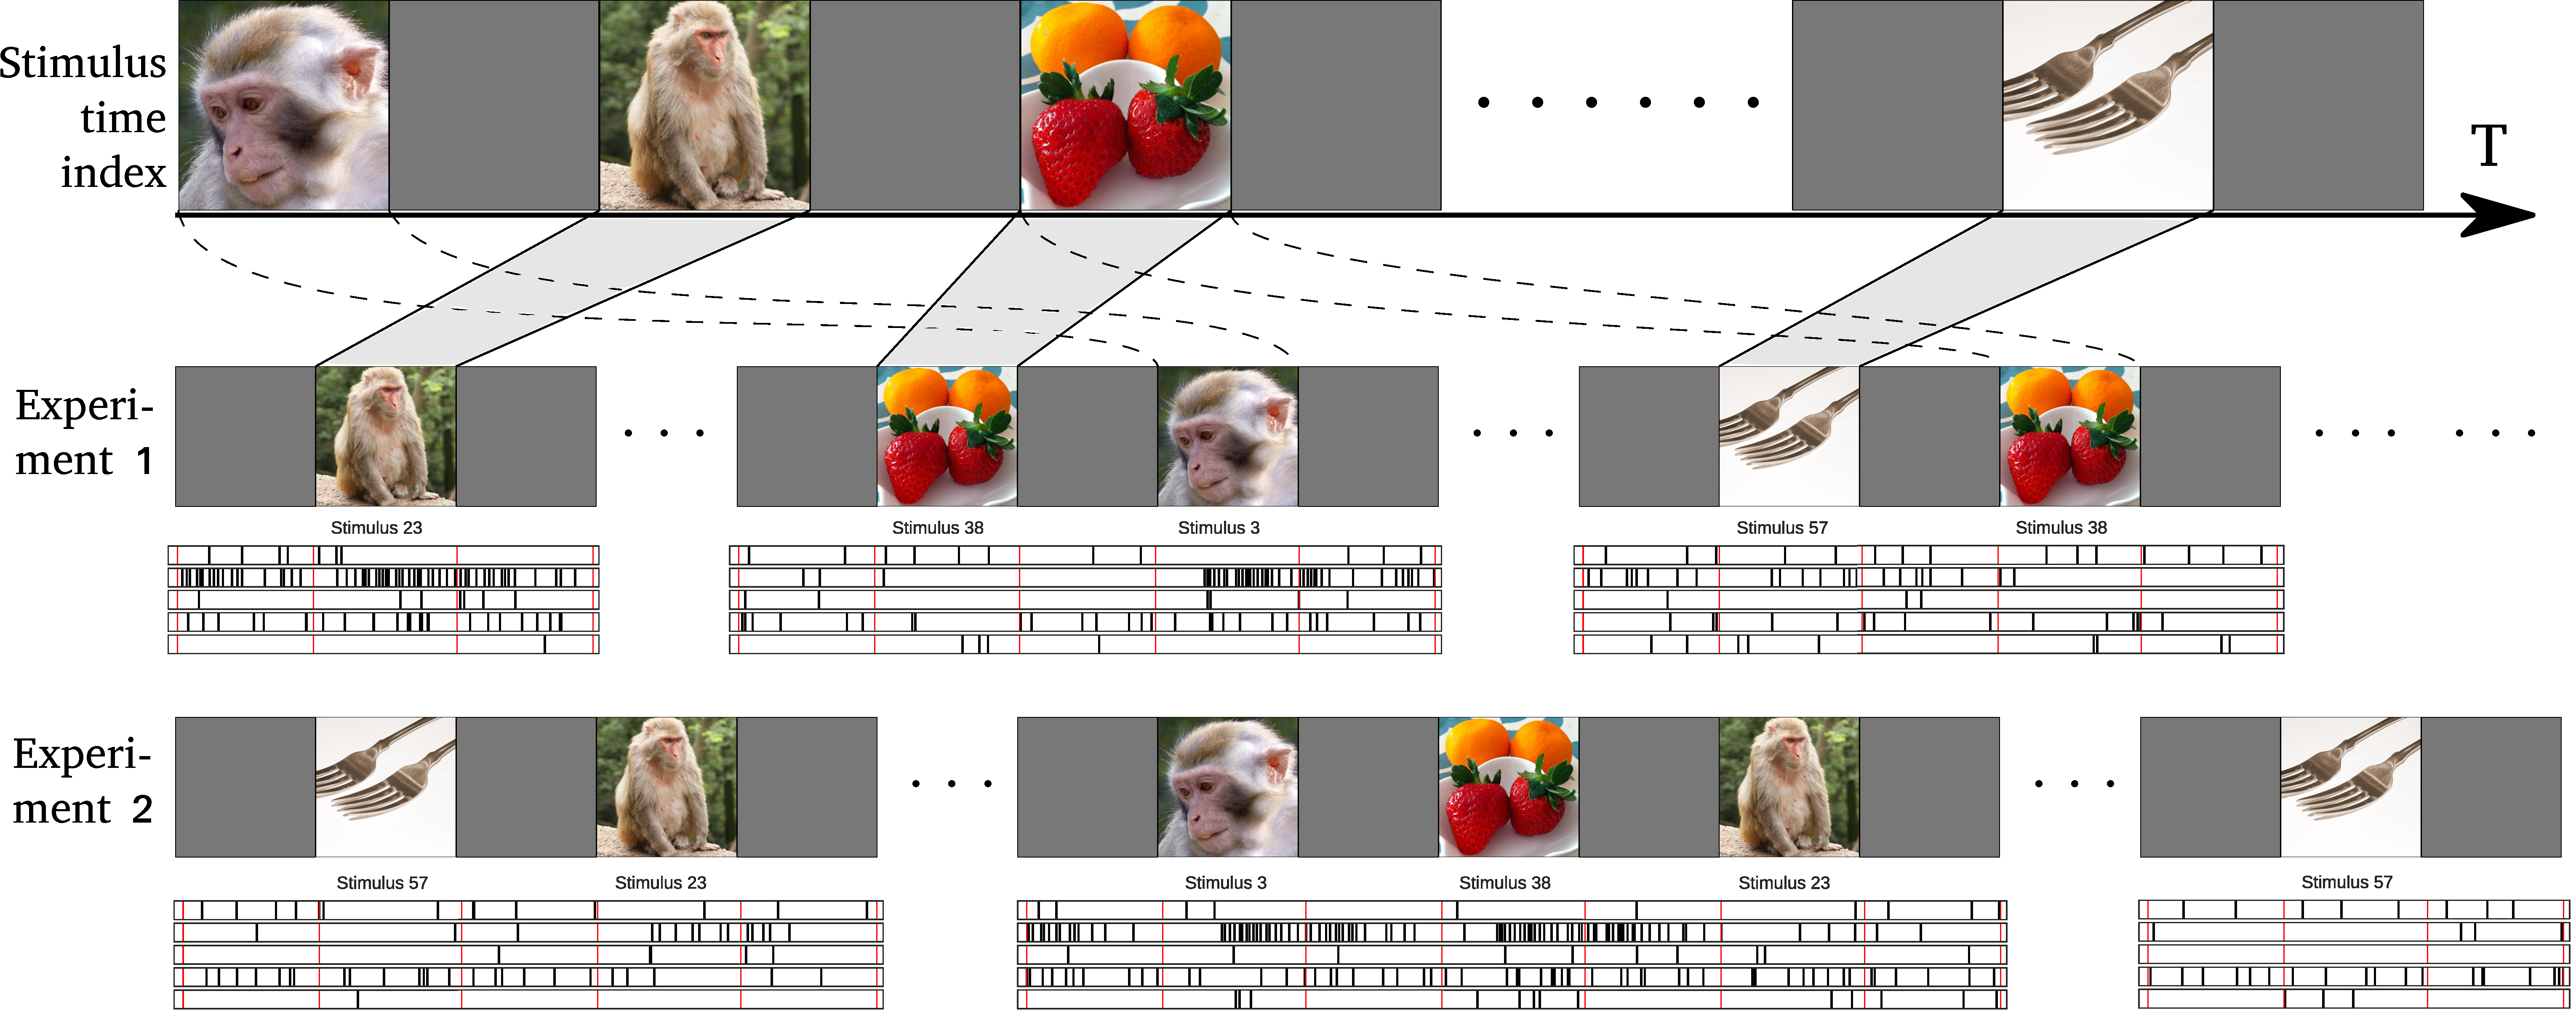
\includegraphics[width=\linewidth]{figures/stim_movie} % this command will be ignored
   \caption{\textbf{Observational model.} A: Stimuli are concatenated to form a single time series indexed by $t$. B: Individual experimental sessions draw from the available set of stimuli, with index $m$ representing unique $(time, unit)$ presentations. Example stimulus sequences for two experiments are shown, with corresponding neuronal spike data. Note that the number of exposure times $M_{tu}$ for each stimulus and unit can be different.}
   \label{fig:movie}
\end{figure}

\section*{Methods}
\label{model_sec}

\subsection{Observation model.}
Consider a population of $U$ spiking neurons or units exposed to a series of stimuli indexed by a time index $t\in \lbrace 1\ldots T\rbrace$. We assume that this time index is unique across all stimuli, such that a particular $t$ represents a unique moment in a particular stimulus. In order to model repeated presentations of the same stimulus to the same neuron, we further assume that each neuron is exposed to a stimulus $M_{tu}$ times, though we do not assume any relationship among $M_{tu}$. That is, we need not assume either that all neurons see each stimulus the same number of times, nor that each stimulus is seen by all neurons. It is thus typical, but not required, that $M_{tu}$ be sparse, containing many 0s, as shown in Figure \ref{fig:movie}.

For each observation $m$ in $M_{tu}$, we then observe a spike count, $N_m$. Note that $m$ is a unique $(time, unit)$ pair that can be denoted by $(t(m), u(m))$. We model these spike counts as arising from a Poisson process with time-dependent rate $\Lambda_{tu}$ and observation-specific multiplicative overdispersion $\theta_m$:
\begin{align}
    \label{obs_model}
    N_{m} &\sim \text{Poisson}(\Lambda_{t(m), u(m)} \theta_m) &
    \text{where} ~~ \theta_m &\sim \text{Gamma}(s_{u(m)}, s_{u(m)})
\end{align}
That is, for a given stimulus presentation, the spiking response is governed by the firing rate $\Lambda$, specific to the stimulus and unit, along with a moment-by-moment noise in the unit's gain, $\theta_m$. We restrict these $\theta_m$ to follow a Gamma distribution with the same shape and rate parameters, since this results in an expected noise gain of 1. In practice, we model this noise as independent across observations, though it is possible to weaken this assumption, allowing for $\theta_m$ to be autocorrelated in time (see Supplement). Note that both the unit and time are functions of the observation index $m$, and that the distribution of the overdispersion for each observation may be specific to the unit observed.

\subsection{Firing rate model.}
At each stimulus time $t$, we assume the existence of $K$ binary latent states $z_{tk}$ and $R$ observed covariates $x_{tr}$. The binary latent states can be thought of as time-varying ``tags'' of each stimulus --- for example, content labels for movie frames --- and are modeled as Markov chains with initial state probabilities $\pi_k$ and transition matrices $A_k$. The observed covariates, by contrast, are known to the experimenter and may include contrast, motion energy, or any other \emph{a priori} variable of interest.

We further assume that each unit's firing rate at a particular point in time can be modeled as arising from the product of three effects: (1) a baseline firing rate specific to each unit ($\lambda_0$), (2) a product of responses to each latent state ($\lambda_z$), and (3) a product of responses to each observed covariate ($\lambda_x$):
\begin{equation}
    \label{fr_model}
    \Lambda_{tu} = \lambda_{0u} \prod_{k = 1}^K (\lambda_{zuk})^{z_{tk}}
    \prod_{r = 1}^R (\lambda_{xur})^{x_{tr}}
\end{equation}
Note that this is conceptually similar to the generalized linear model for firing rates (in which we model $\log \Lambda$) with the identification $\beta = \log \lambda$. However, by modeling the firing rate as a product and placing Gamma priors on the individual effects, we will be able to take advantage of closed-form variational updates resulting from conjugacy that avoid explicit optimization (see below). Note also, that because we assume the $z_{tk}$ are binary, the second term in the product above simply represents the cumulative product of the gain effects for those features present in the stimulus at a given moment in time.

In addition, to enforce parsimony in our feature inference, we place sparse hierarchical priors with hyperparameters $\gamma = (c, d)$ on the $\lambda_z$ terms:
\begin{align}
    \label{hierarchy}
    \lambda_{zuk} &\sim \text{Gamma}(c_{zk}, c_{zk} d_{zk}) & c_{zk} &\sim \text{Gamma}(a_{ck}, b_{ck})
    & d_{zk} &\sim \text{Gamma}(a_{dk}, b_{dk})
\end{align}
That is, the population distribution for the responses to latent features is a gamma distribution, with parameters that are themselves gamma-distributed random variables. As a result, $\mathbb{E}[\lambda_u] = d^{-1}$ and $\text{var}[\lambda_u] = (cd^2)^{-1}$, so in the special case of $c$ large and $d\sim \mathcal{O}(1)$, the prior for firing rate response to each latent feature will be strongly concentrated around gain 1 (no effect). As we show below, this particular choice results in a model that only infers features for which the data present strong evidence, controlling for spurious feature detection. In addition, this particular choice of priors leads to closed-form updates in our variational approximation. For the baseline terms, $\lambda_{0u}$, we use a non-sparse version of the same model; for the covariate responses, $\lambda_{xu}$, we model the unit effects non-hierarchically, using independent Gamma priors for each unit.

Putting all this together, we then arrive at the full generative model:
\begin{align}
    p(N, \Lambda, \theta) &= p(N| \Lambda, \theta)p(\Lambda|\lambda, z)
    p(\lambda|\gamma) p(\gamma)
    p(z|A, \pi)
    p(A)p(\pi)p(\theta|s)p(s)
\end{align}
with $p(\lambda|\gamma) = \prod_u p(\lambda_{0u}|c_0, d_0)\prod_{kr} p(\lambda_{zuk}|c_{zk}, d_{zk}) p(\lambda_{xur})$ and $p(\gamma) = p(c_0)p(d_0)\prod_k p(c_{zk}) p(d_{zk})$ in conjunction with the definitions of $p(N|\Lambda, \theta)$ and $\Lambda(\lambda, z, x)$ in Eq (\ref{obs_model}) and (\ref{fr_model}). The generative model for spike counts is illustrated in Figure \ref{fig1}.

% Place figure captions after the first paragraph in which they are cited.
\begin{figure}
    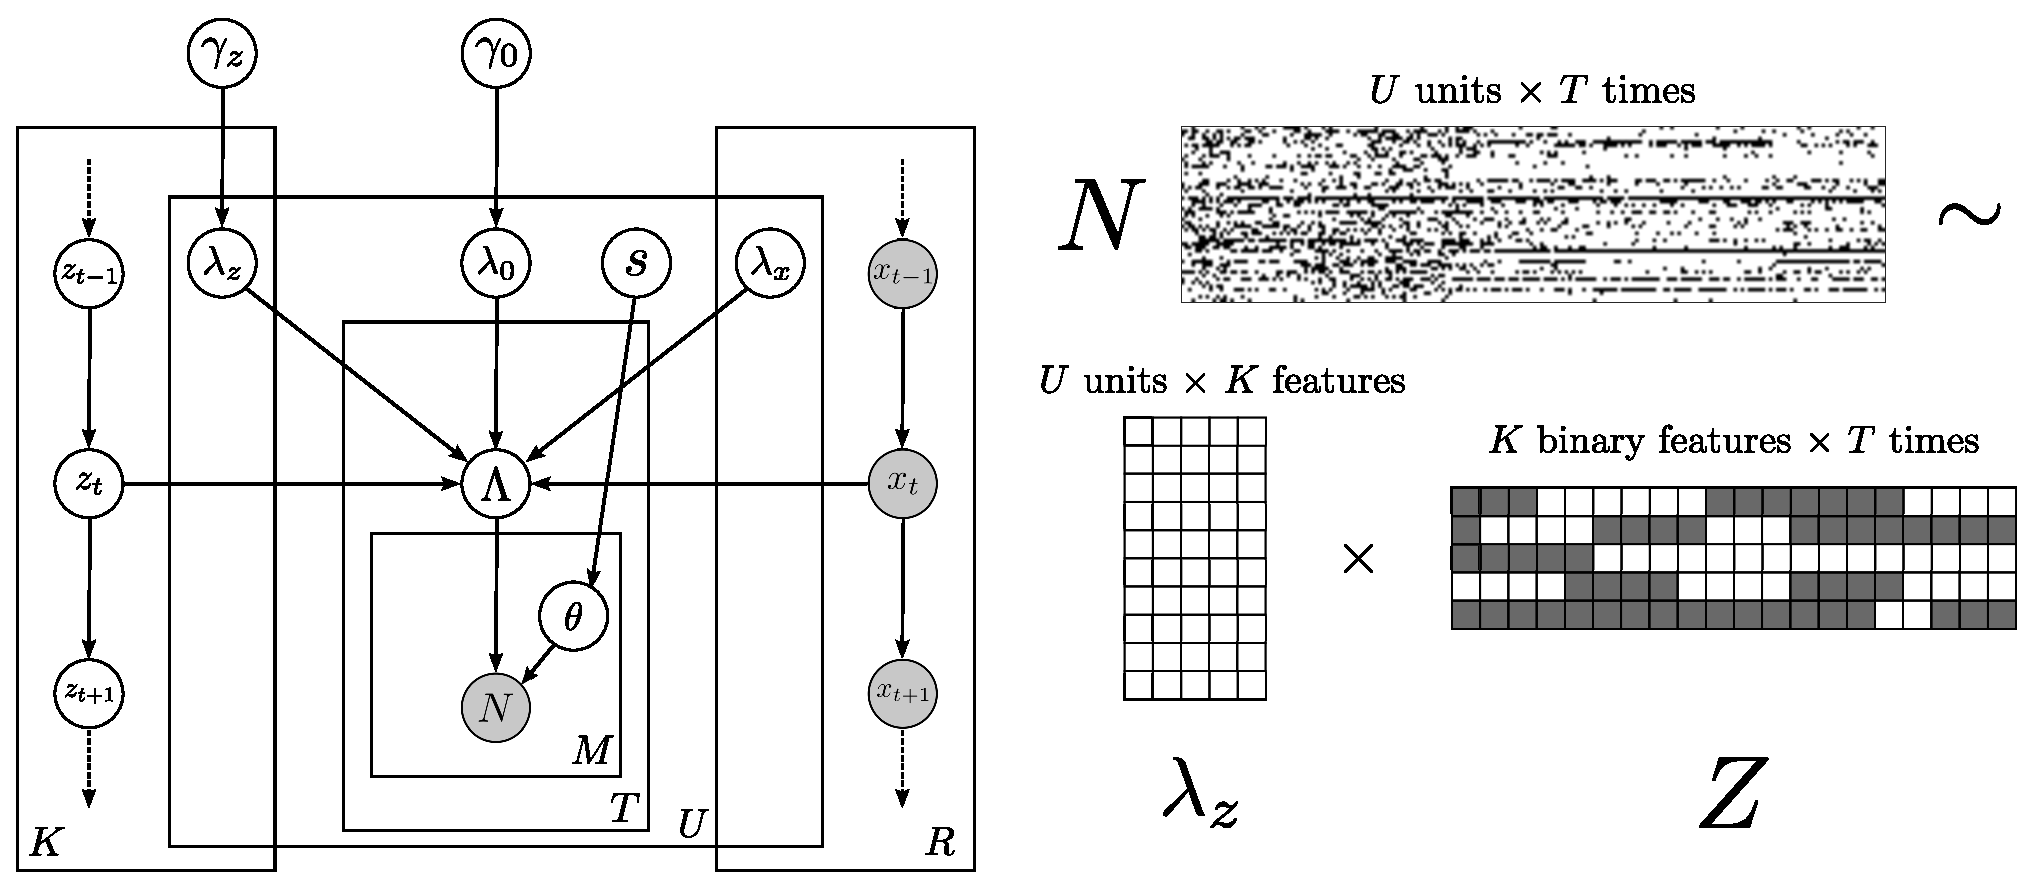
\includegraphics[width=\linewidth]{figures/model}
	\caption{\textbf{Generative model for spike counts.}
	A: Counts are assumed Poisson-distributed, with firing rates $\Lambda$ that depend on each unit's responses ($\lambda$) to both latent discrete states $z_t$ and observed covariates $x_t$ that change in time, as well as a baseline firing rate $\lambda_0$. $\gamma$ nodes represent hyperparameters for the firing rate effects. $\theta$ is a multiplicative overdispersion term specific to each observation, distributed according to hyperparameters $s$. B: Spike counts $N$ are observed for each of $U$ units over stimulus time $T$ for multiple presentations $M_{tu}$.}
\label{fig1}
\end{figure}

\subsection{Inference.}
Given a sequence of stimulus presentations $(t(m),u(m))$ and observed spike counts $N_m$, we want to infer both the model parameters $\Theta = (\lambda_0, \lambda_z, \lambda_x, A, \pi, c_0, d_0, c_z, d_z, s)$ and latent variables  $Z=(z_{kt},\theta_m)$. That is, we wish to calculate the joint posterior density:
\begin{equation}
    p(\Theta,Z|N) \propto p(N | Z, \Theta) p(Z) p(\Theta)
\end{equation}
In general, calculating the normalization constant for this posterior is computationally intractable. Instead, we will use a variational approach, approximating $p(\Theta, Z|N)$ by a variational posterior $q(Z, \Theta) = q_Z(Z) q_\Theta(\Theta)$ that factorizes over parameters and latents but is nonetheless close to $p$ as measured by the Kullback-Leibler divergence \cite{Wainwright2008-ii}. Equivalently, we wish to maximize the variational objective
\begin{equation}
    \label{elbo}
    \mathcal{L} \equiv \mathbb{E}_q \left[\log \frac{p(\Theta,Z|N)}{q(\Theta, Z)} \right] = \mathbb{E}_q \left[\log p(\Theta,Z|N) \right] + \mathcal{H}[q_\Theta(\Theta)] + \mathcal{H}[q_Z(Z)]
\end{equation}
with $\mathcal{H}$ the entropy. We adopt the factorial HMM trick \cite{ghahramani1997factorial}, making the reasonable assumption that the posterior factorizes over each latent time series $z_{\bigcdot k}$ and the overdispersion factor $\theta_m$, as well as the rate parameters $\lambda_{\bigcdot u \bigcdot}$ associated with each Markov process. Thus the variational objective decomposes in a natural way, and choices are available for nearly all of the $q$'s that lead to closed-form updates.
%This factorization results in a variational posterior of the form:
%\begin{multline}
%    q(\Theta,Z) = q(c_0)q(d_0)\prod_m q(\theta_m) \prod_u q(s_u) q(\lambda_{0u}) \prod_r q(\lambda_{xur}) \times \\
%    \prod_k q(c_k) q(d_k)
%    q(\lambda_{zuk}) q(c_{zk}) q(d_{zk}) q(z_k) q(\pi_k) q(A_k)
%\end{multline}
%With this ansatz, the variational objective decomposes in a natural way, and choices are available for nearly all of the $q$s that lead to closed-form updates.

\subsection{Variational posterior.}
Substituting Eq (\ref{fr_model}) into Eq (\ref{obs_model}), we can write and brake down the probability of the observed data $N$ as
\begin{multline}
    \label{log_evidence}
    \log p(N, z|x, \Theta) = \sum_{mkr} \left[
        N_m \left( \log \theta_m +
            \log \lambda_{0u(m)} +
            z_{t(m) k} \log \lambda_{zu(m) k} +
            x_{t(m) r} \log \lambda_{xu(m) r}
            \right)
    \right] \\
    - \sum_m \theta_m \Lambda_{t(m) u(m)} +
    \sum_{mk} \log (A_k)_{z_{t(m)+1, k}, z_{t(m), k}} +
    \sum_k \log (\pi_k)_{z_{0k}} + \text{constant,}
\end{multline}
where again, $m$ indexes observations of $(t(m),u(m))$ pairs and the last two nontrivial terms represent the probability of the Markov sequence given by $z_{tk}$. Given that Eq (\ref{log_evidence}) is of an exponential family form for $\theta$ and $\lambda$ when conditioned on all other variables, free-form variational arguments \cite{Wainwright2008-ii} suggest variational posteriors:
\begin{align}
    \lambda_{0u} &\sim \text{Gamma}(\alpha_{0u}, \beta_{0u}) &
    \lambda_{zuk} &\sim \text{Gamma}(\alpha_{zuk}, \beta_{zuk}) &
    \lambda_{xur} &\sim \text{Gamma}(\alpha_{xur}, \beta_{xur})
\end{align}
For the first of these two, updates in terms of sufficient statistics involving expectations of $\gamma = (c, d)$ are straightforward (see Supplement). However, this relies on the fact that $z_t \in \lbrace0, 1\rbrace$. The observed covariates $x_t$ follow no such restriction, which results in a transcendental equation for the $\beta_x$ updates. In our implementation of the model, we solve this using an explicit BFGS optimization on each iteration. Moreover, we place non-hierarchical Gamma priors on these effects: $\lambda_{xur} \sim \text{Gamma}(a_{xur}, b_{xur})$.

For each latent variable $z$, the Markov Chain parameters $\pi_k$ and $A_k$, together with the observation model Eq (\ref{log_evidence}) determine a Hidden Markov Model, for which inference can be performed efficiently via conjugate updates and the well-known forward-backward algorithm \cite{beal2003variational}. More explicitly, given $\pi$, $A$, and the emission probabilities for the observations, $\log p(N|z)$, the forward-backward algorithm returns the probabilities $p(z_t=s)$ (posterior marginal), $p(z_{t+1} =s', z_t=s)$ (two-slice marginal) and $\log Z$ (normalizing constant).

\section*{Results}
\subsection{Inferred states from synthetic data.}
To test the model performance on discrete states data, we generated synthetic data from $U=100$ neurons for $T=10,000$ time bins of $dt=0.0333s$ ($\approx 6$min of movie at 30 frames per second). Assumed firing rates and effect sizes were realistic for cortical neurons, with mean baseline rates of 10 spikes/s and firing rate effects given by a $\text{Gamma}(1, 1)$ distribution for $K_{\text{data}}=3$ latent features. In addition, we included $R=3$ known covariates generated according to Markov dynamics. For this experiment, we assumed that each unit was presented only once with the stimulus time series, so that $M_{tu} = 1$. That is, we tested a case in which inference was driven primarily by variability in population responses across stimuli rather than pooling of data across repetitions of the same stimulus. Moreover, to test the model's ability to parsimoniously infer features, we set $K=5$. That is, we asked the model to recover more features than were present in the data. In reality, this is not necessarily true because in most cases data are highly redundant thus can be represented with much smaller number of features. Finally, we placed hierarchical priors on neurons' baseline firing rates and sparse hierarchical priors on firing rate effects of latent states. We used 5 random restarts and iterated over parameter updates until the fractional change in evidence lower bound $\mathcal{L}$ (see supplement) dropped below $10^{-4}$ to ensure it is converging.

As seen in Figure \ref{synthetic}, the model correctly recovers the features present in the original data. We quantified this by calculating the normalized mutual information $\hat{I}\equiv I(X, Y)/\sqrt{H(X)H(Y)}$, between the actual states and the inferred states, with $H(Z)$ and $I$ estimated by averaging the variational posteriors (both absolute and conditioned on observed states) across time. Note that superfluous features in the model have high posterior uncertainty for $z_k$ and high posterior confidence for $\lambda_{zk}$ around 1 (no effect). In addition, the model correctly recovers coefficients for the observed covariates, and when limited to fewer features than in the generating model, recovers a subset of the features accurately rather than blending features together (Figure \ref{synthetic}).

% Place figure captions after the first paragraph in which they are cited.
\begin{figure}
    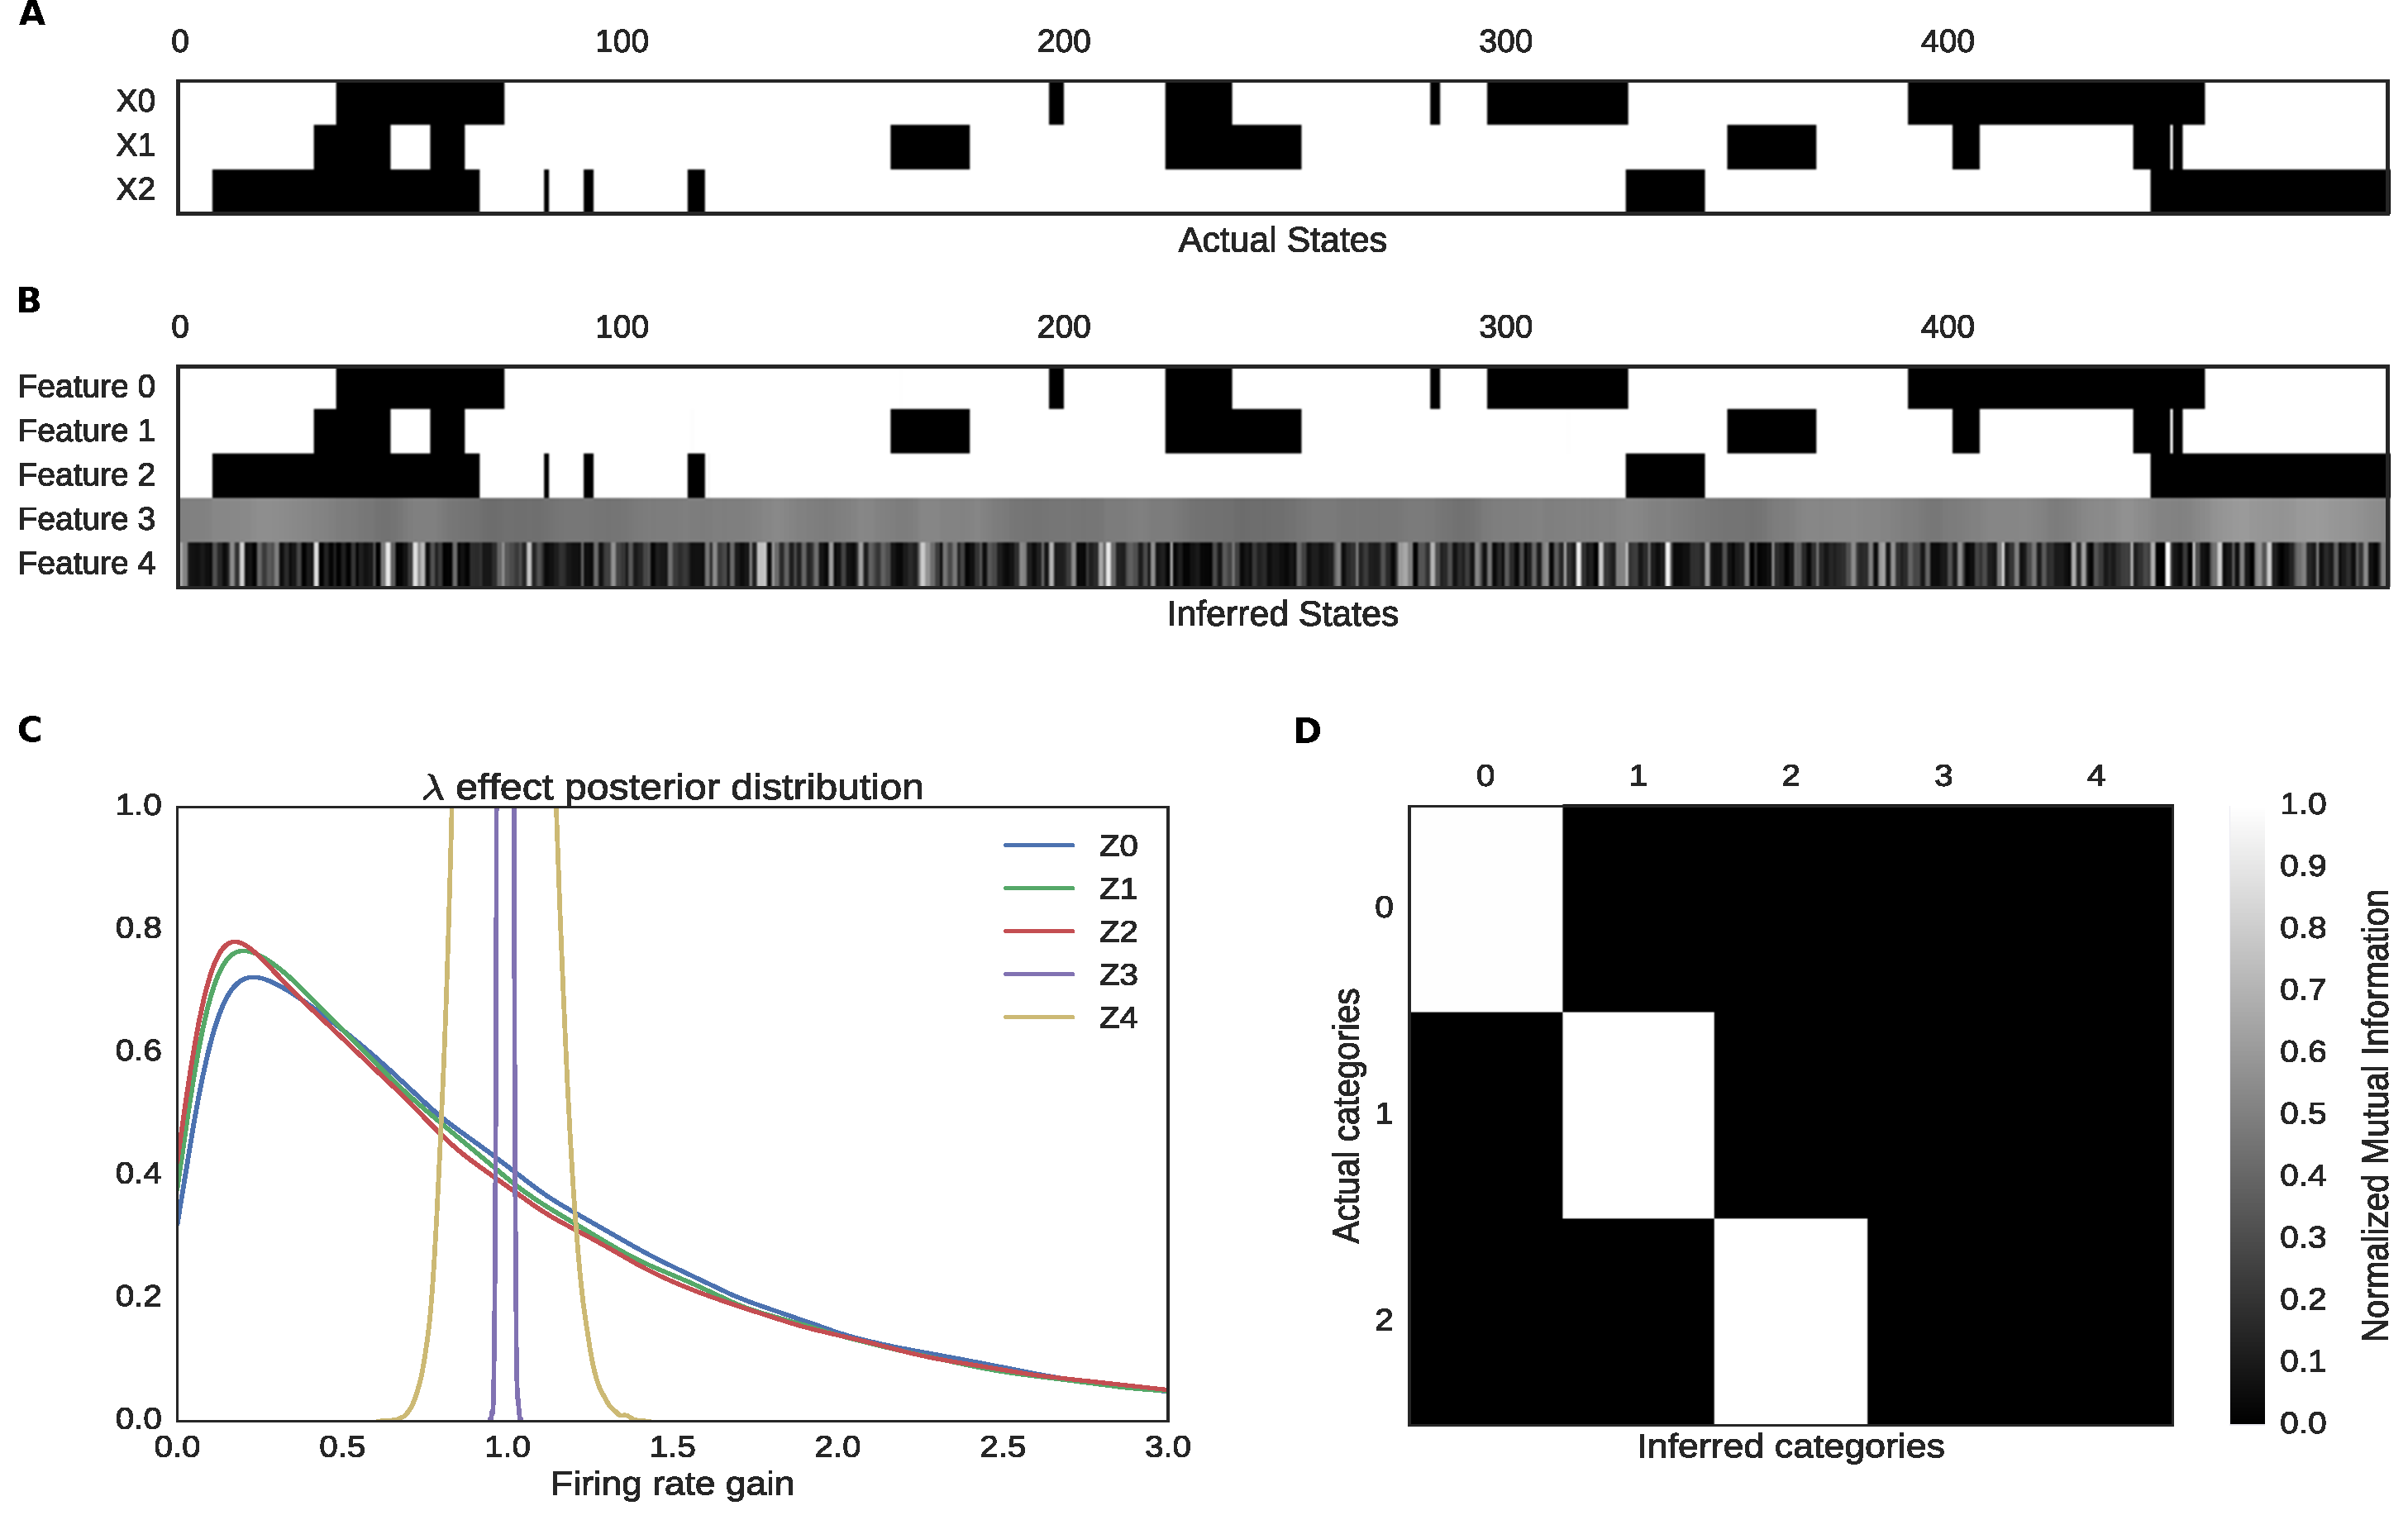
\includegraphics[width=\linewidth]{figures/synthetic}
	\caption{\textbf{Comparison of actual and inferred states of the synthetic data.} A: Actual features for a subset of stimulus times in the synthetic dataset. B: Recovered binary features for the same subset. Features have been reordered for display. The unused features are in gray, indicating a high posterior uncertainty in the model. C: Population posterior distributions for inferred hyper parameters. Features 3 and 4 are effectively point masses around gain 1 (no effect), while features 0--2 approximate the $\text{Gamma}(1, 1)$ data-generating model. D: Normalized mutual information between actual and inferred states.}
	\label{synthetic}
\end{figure}

\subsection{Inferred firing rates in time for labeled neural data.}
In order to test the model performance on long time correlated neural activities, we applied our model to a well-studied neural data set comprising single neuron recordings from macaque area LIP collected during the performance of a perceptual discrimination task \cite{roitman2002response}\footnote{Data available at \texttt{https://www.shadlenlab.columbia.edu/resources/RoitmanDataCode.html}}. In the experiment, stimuli consisted of randomly moving dots, some percentage of which moved coherently in either the preferred or anti-preferred direction of motion for each neuron. The animal's task was to report the direction of motion. Thus, in addition to 5 coherence levels, each trial also varied based on whether the motion direction corresponded to the target in or out of the response field as depicted in Fig. \ref{roitman}.\footnote{In the case of 0\% coherence, the direction of motion was inherently ambiguous and coded according to the monkey's eventual choice.}

We fit a model with $K = 10$ features and $U = 27$ units to neural responses from the 1-second stimulus presentation period of the task. Spike counts corresponded to bins of $dt = 20$ms. For this experiment, units were individually recorded, so each unit experienced a different number of presentations of each stimulus condition, implying a ragged observation matrix. As a result, this dataset tests the model's ability to leverage shared task structure across multiple sessions of recording, demonstrating that simultaneously recorded units are not required for inference of latent states.

Figure \ref{roitman} shows the experimental labels from the concatenated stimulus periods, along with labels inferred by our model. Once again, the model has left some features unused, but correctly discerned differences between stimuli in the unlabeled data. Even more importantly, though given the opportunity to infer ten distinct stimulus classes, the model has made use of only five. Moreover, the discovered features clearly recapitulate the factorial design of the experiment, with the two most prominent features, $Z_1$ and $Z_2$, capturing complementary values of the variable with the largest effect in the experiment: whether or not the relevant target was inside our outside the receptive field of the recorded neuron. This difference can be observed in both the averaged experimental data and the predicted data from the model (see Figure \ref{roitman}.C), where the largest differences are between the dotted and solid lines.

But the model also reproduces less obvious features: it correctly discriminates between two identical stimulus conditions (0\% coherence) based on the monkey's eventual decision (In vs Out). In addition, the model correctly captures the initial 200ms ``dead time'' during the stimulus period, in which firing rates remain at pre-stimulus baseline. (Note that the timing is locked to the stimulus and consistent across trials, not idiosyncratic to each trial as in \cite{Latimer2015-pb}.) Finally, the model resists detection of features with little support in the experimental data. For instance, while feature $Z_4$ captures the large difference between 50\% coherence and other stimuli, the model does not infer a difference between intermediate coherence levels that are indistinguishable in this particular dataset. That is, mismatches between ground truth labels and model-inferred features here reflect underlying ambiguities in the neural data, while the model's inferred features correctly pick out those combinations of variables most responsible for differences in spiking across conditions.

% Place figure captions after the first paragraph in which they are cited.
\begin{figure}
    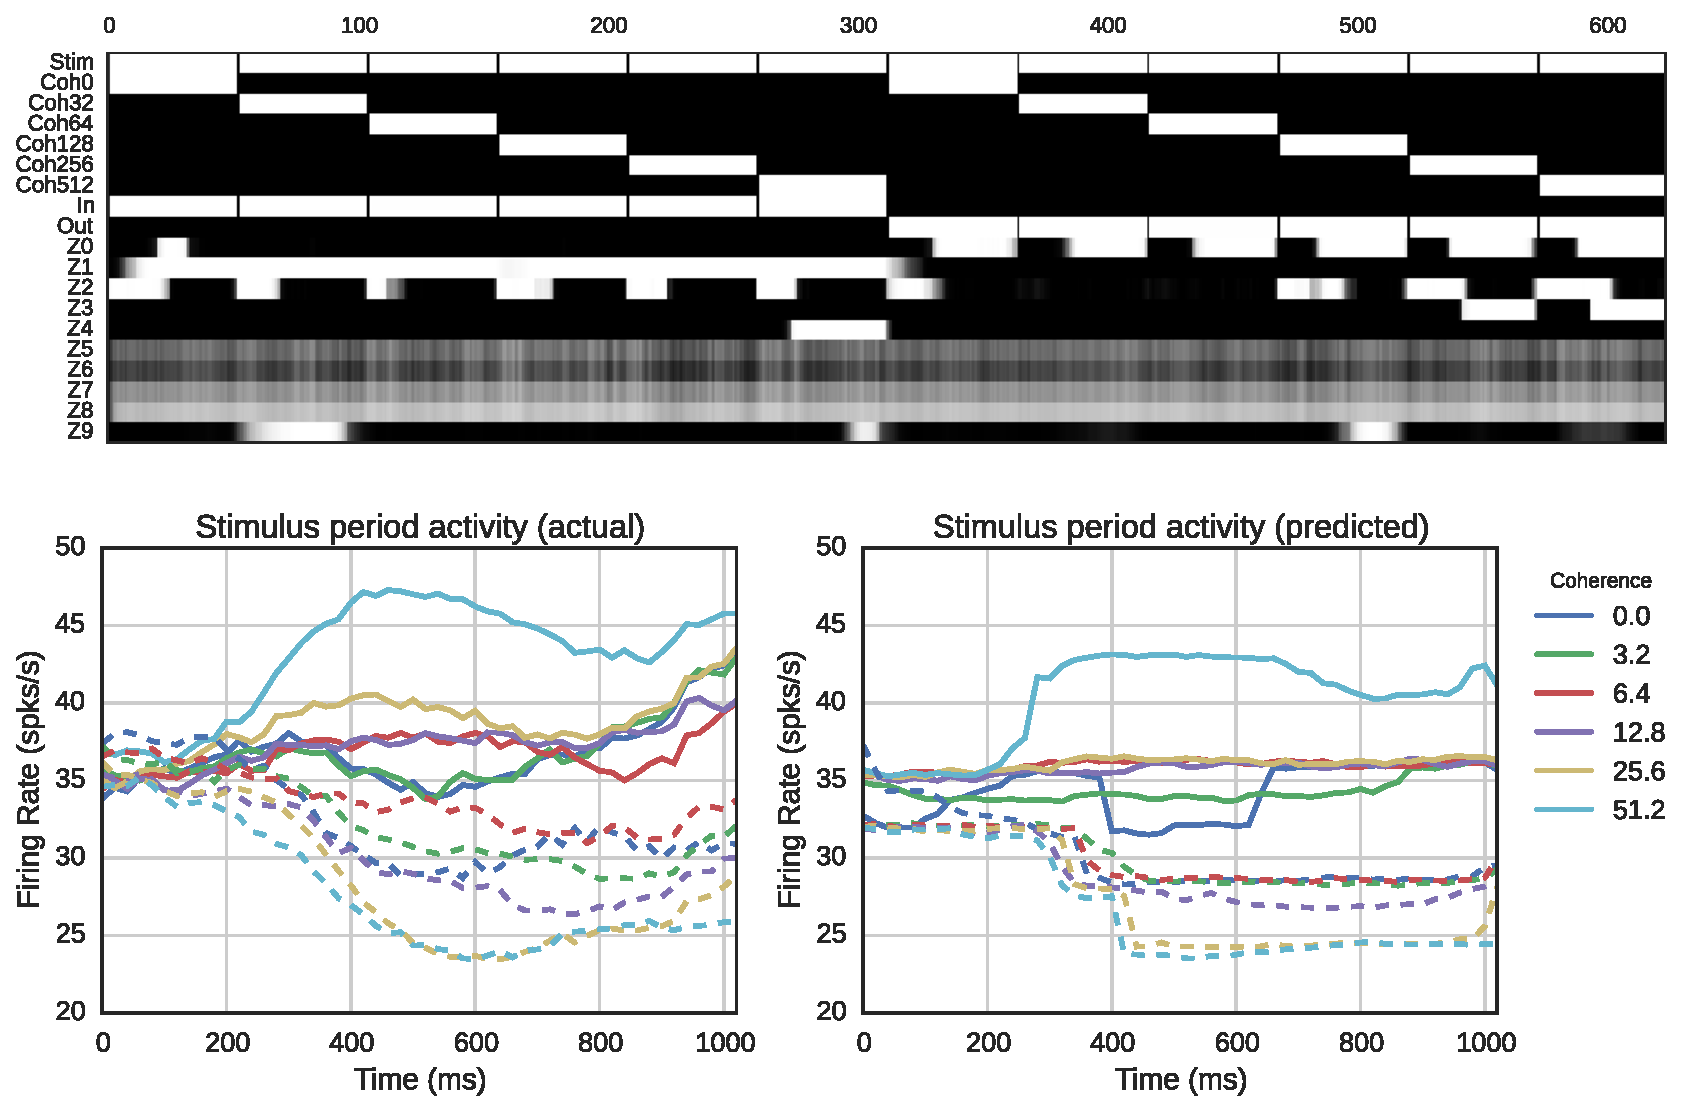
\includegraphics[width=\linewidth]{figures/roitman}
	\caption{\textbf{Comparison of actual and inferred states of the Roitman dataset.}
	A: Indicators of actual categories represented in the stimulus presentation period. The categories are not independent of each other. Stimuli are joined sequentially, labeled by a single, unique stimulus time. B: Recovered binary features during the stimulus presentation period. Note that model features 6 -- 9 are unused and that Features 1 \& 2 closely track the In and Out features of the data, respectively. C: Actual and predicted firing rates for the stimulus period. Note that the model infers stimulus categories from the data, including appropriate timing of differentiation between categories.}
	\label{roitman}
\end{figure}

\subsection{Inferred categories of image stimuli from visual category data.}
\label{it_neuron_expt}
As a second test of our model, we applied our algorithm to a designed structured stimuli dataset comprising $U = 56$ neurons from macaque inferotemporal cortex \cite{McMahon2014-qq} to test its performance on finding the actual categories of stimuli. These neurons were repeatedly presented with 96 stimuli comprising 8 categories ($M$ = 1483 total trials, with each stimulus exposed between 12 to 19 times to each unit) comprising monkey faces, monkey bodies, whole monkeys, natural scenes, food, manmade objects, and patterns (Figure \ref{fig:imgclust}.A). Data consisted of spike time series, which we binned into a 300ms pre-stimulus baseline, a 300ms stimulus presentation period, and a 300ms post-stimulus period. Three trials were excluded because of the abnormal stimulus presentation period. To maximize interpretability of the results, we placed strong priors on the $\pi_k$ to formalize the assumption that all features were off during the baseline period. We also modeled overdispersion with extremely weak priors to encourage the model to attribute fluctuations in firing to noise in preference to feature detection. We again fit $K = 10$ features with sparse hierarchical priors on population responses.

The inferred categories based on binned population responses are shown in Figure \ref{fig:imgclust}.B. For clarity, here we only show population mean effects with modulation gain greater than 5\%, though the full set of inferred states can be found in Figure \ref{fig:imgclust_sub}. Out of the original categories, our model successfully recovers three features clearly corresponding to categories involving monkeys (Features 0 -- 2). These can be viewed additively, with Feature 0 exclusive to monkey face close-ups, Feature 1 any photo containing a monkey face, either near or far; and Feature 2 any image containing a monkey body part including faces. Given the nature of the model, it may be better to view these as a ``combinatorial'' code, with monkey close-ups encoded as $0\& 1\& 2$ ($\sim 59.46\%$ increase in firing), whole monkeys as $1 \& 2$ ($\sim 32.47\%$ increase), and monkey body parts as $2$ ($\sim 7.62\%$ increase). Of course, this is consistent with what was found in \cite{McMahon2014-qq}, though our model used no labels on the images. And our interpretation that these neurons are sensitive to close-ups and faraway face and body parts is consistent with findings by another study using different experimental settings \cite{McMahon5537}.

Again, as noted above, our results in Figure \ref{fig:imgclust}.A and \ref{fig:imgclust}.B indicate predicted population responses, derived from the hierarchical prior. As evidenced in Figure \ref{fig:imgclust}.C and \ref{fig:imgclust}.D, individual neuron effects could be much larger. These panels show data for two example units, along with the model's prediction. Clearly, the model recapitulates the largest distinctions between images in the data, though the assumption that firing rates should be the same for all images with similar features fails to capture some variability in the results. Even so, uncertainties in the predicted firing rates are also in line with uncertainties from those of observed rates, indicating that our model is correctly accounting for trial-to-trial noise.

% Place figure captions after the first paragraph in which they are cited.
\begin{figure}
    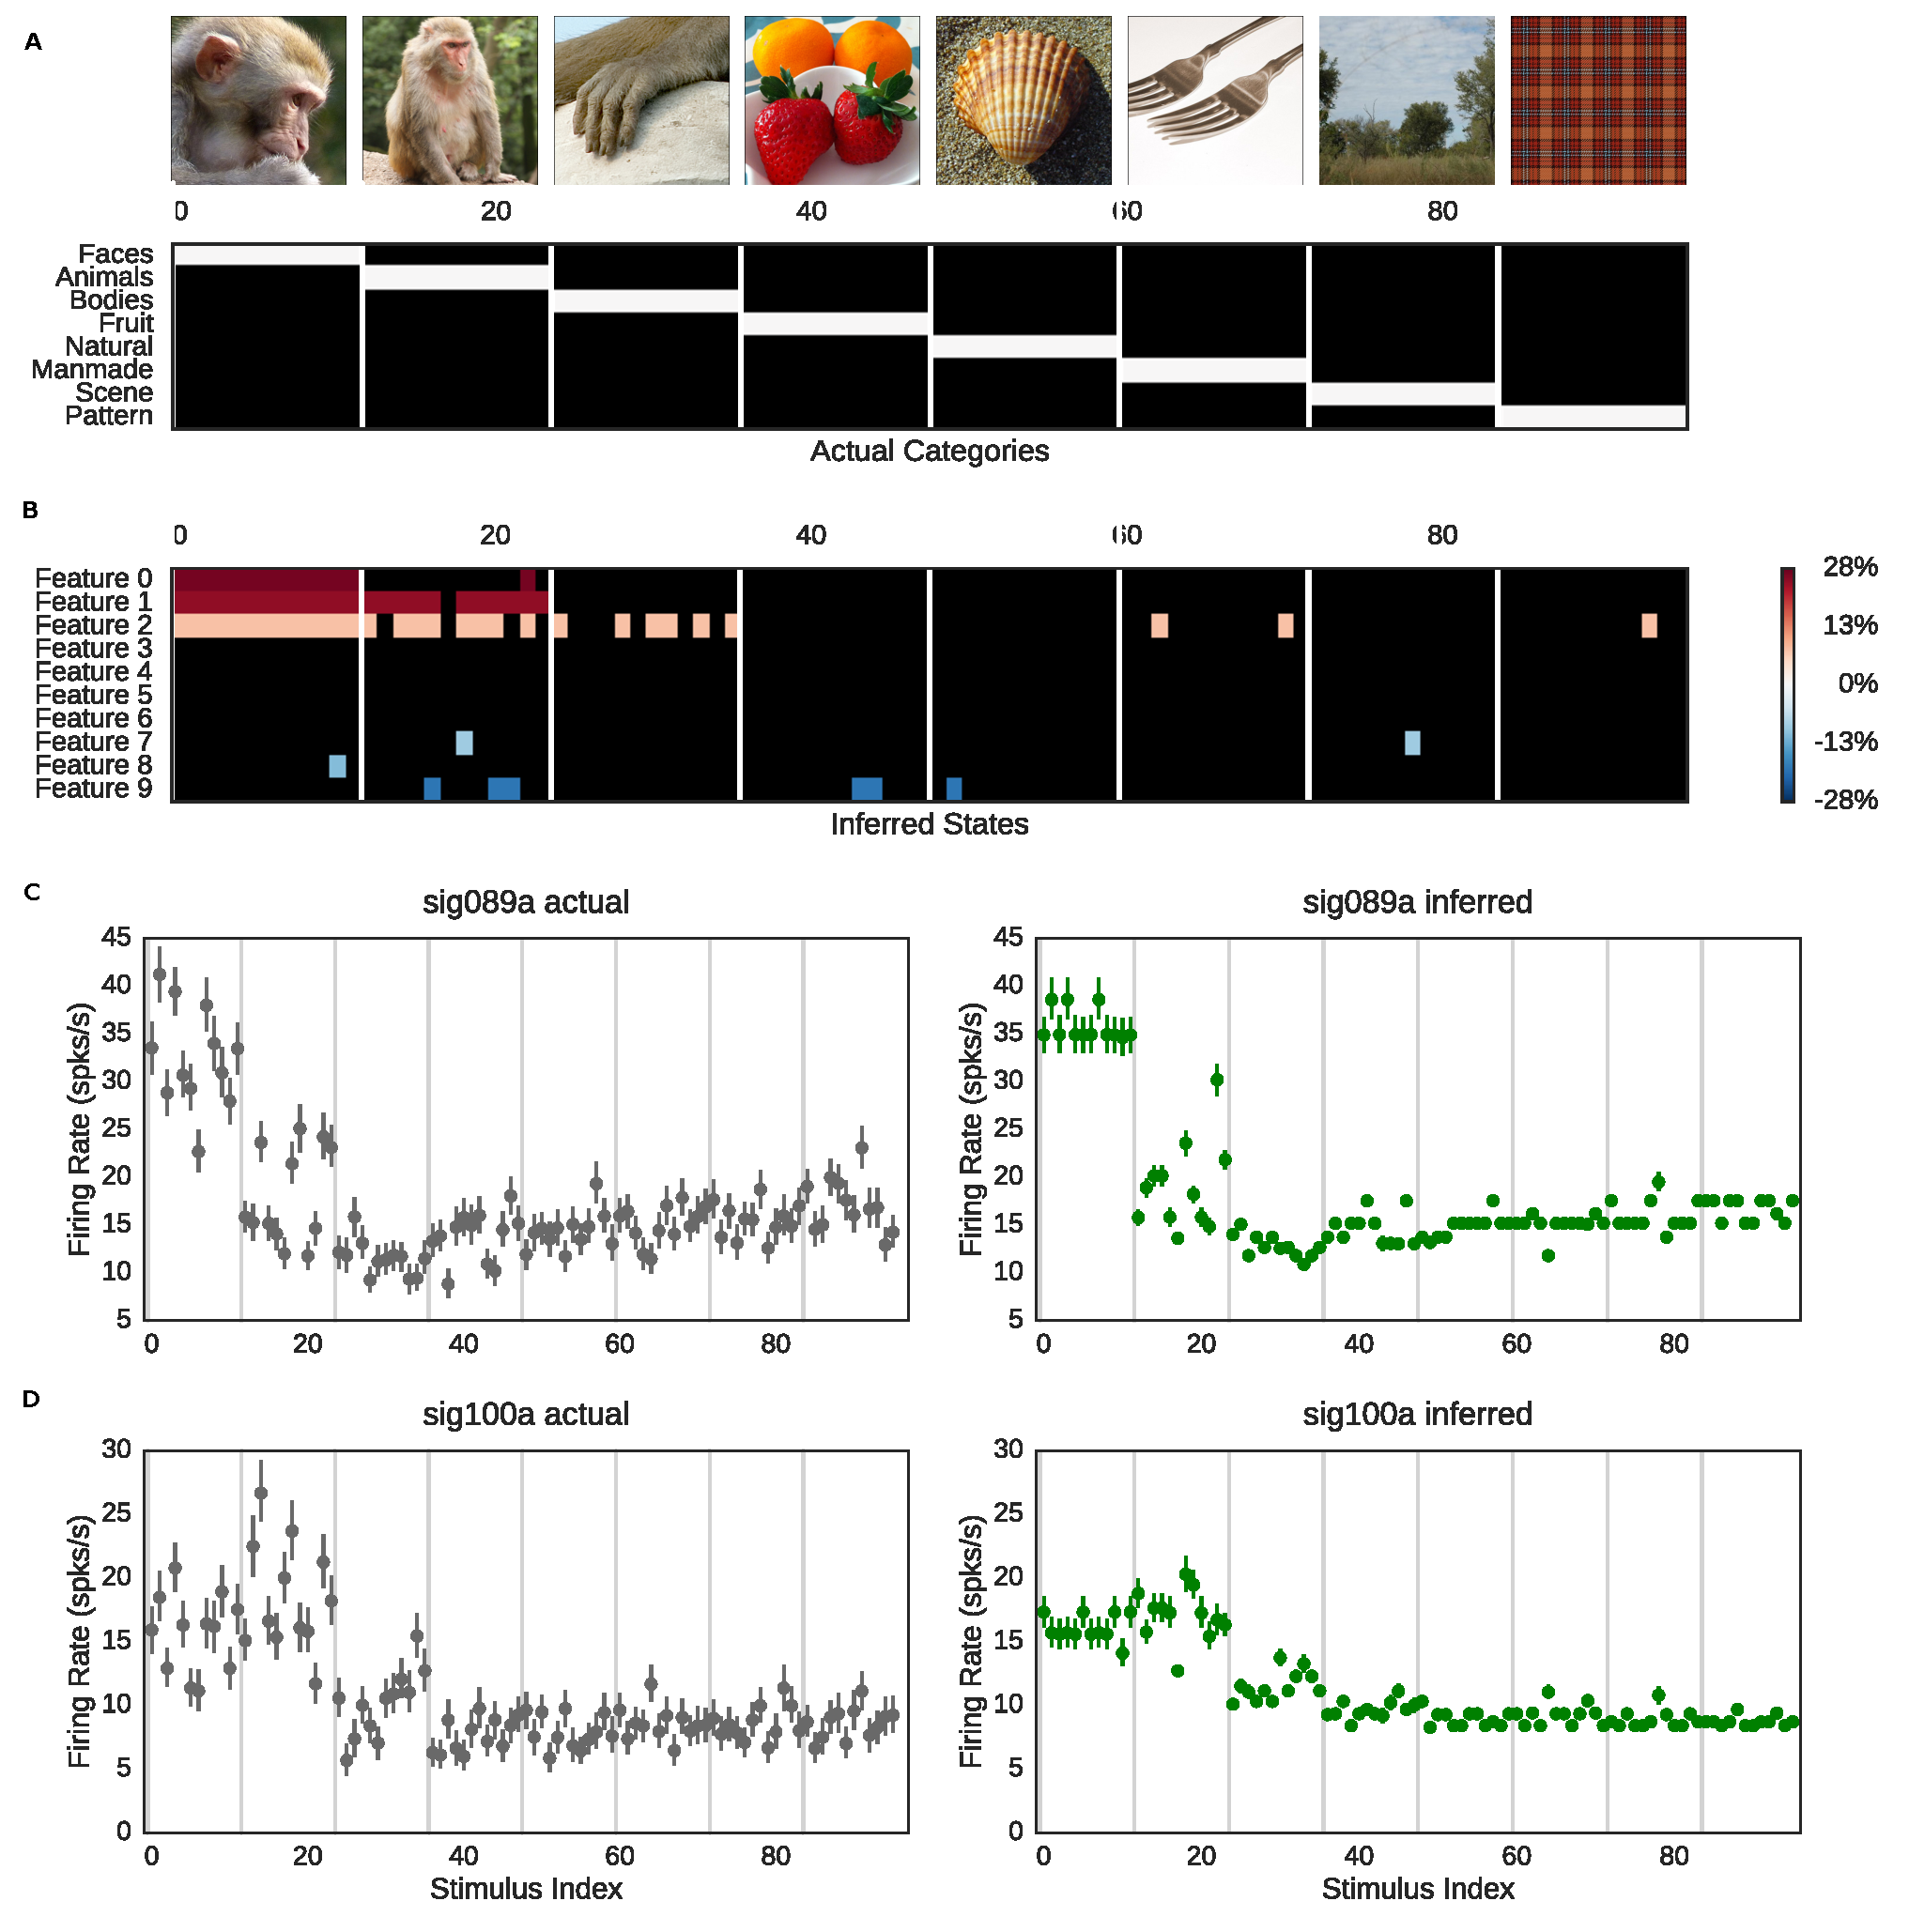
\includegraphics[width=\linewidth]{figures/imgclust}
	\caption{\textbf{Comparison of actual and inferred states of the macaque dataset.}
	\linespread{1.2} \small A: Actual categories in the macaque data set. B: The inferred states from our model. The color represents the multiplicative effect to the population baseline firing rates. Note that our model shows a clear increase of firing rates in the categories of monkey faces, whole monkeys, and some stimuli within monkey bodies. C: Actual and predicted spikes per second across all stimulus of neuron 089a. D. Actual and predicted spikes per second across all stimulus of neuron 100a. Error bars for data represent 95\% credible intervals for the firing rate based on observed data under a Poisson model with weak priors. Error bars on predictions are 95\% credible intervals based on simulation from the approximate posterior for the given unit.
    }
	\label{fig:imgclust}
\end{figure}

Finally, even the weaker, sparser features inferred by our model captured intriguing additional information. As shown in Figure \ref{fig:imgclust_sub}, Feature 4, a feature only weakly present in the population as a whole (and thus ignored in \ref{fig:imgclust_sub}.A), when combined with the stronger Features 0, 1, and 2, successfully distinguishes between the monkey close-ups with direct and averted gaze. (Stimulus 5, with averted gaze, is additionally tagged with Feature 5, which we view as an imperfect match.) Thus, despite the fact that Feature 4 is barely a 3.4\% gain change over the population, it suggests a link between neural firing and gaze direction, one for which there happens to be ample evidence \cite{Perrett23, Freiwald845}. Similarly, Feature 5, barely a 1.1\% effect, correctly tags three of the four close-ups with rightward gaze (with one false positive). Clearly, neither of these results is dispositive in this particular dataset, but in the absence of hypotheses about the effect of head orientation and gaze on neuronal firing, these minor features might suggest hypotheses for future experiments.

% Place figure captions after the first paragraph in which they are cited.
\begin{figure}
    \includegraphics[width=\linewidth]{figures/imgclust_subgroups}
	\caption{\textbf{Small features suggest additional neural hypotheses.}
	A: Zoomed-in view of Figure \ref{fig:imgclust}.A, focusing on the first 24 images. B: The feature combinations 0\&1\&2 (Group 1) and 0\&1\&2\&4 (Group 2) are distinguished by direct vs. indirect gaze. Stimulus 5, which is coded 0\&1\&2\&5, may be considered a false negative.}
	\label{fig:imgclust_sub}
\end{figure}

An additional feature of our approach is that the generated labels provide a concise and fairly complete summary of the stimulus-related activity of all neural recordings, which can be observed by comparing the categorization performance of decoded neural activity to the categorization performance of the decoded features. Although our model is not a data compression method, it nonetheless preserves most of the information about image category contained in the $N=56$ dimensional spike counts via a 10-dimensional binary code. That is, using a sparse logistic regression on two-bit combinations of our features to predict stimulus category ties and outperforms, respectively a multinomial logistic regression on the raw spike counts (see Supplement).

\section*{Discussion}



In this paper, we have proposed and implemented a method for learning features in stimuli via the responses of populations of spiking neurons. This work addresses a growing trend in systems neuroscience --- the increasing use of rich and unstructured or structured stimulus sets --- without requiring either expert labeling or a metric on the stimulus space. As such, we expect it to be of particular use in disciplines like social neuroscience, olfaction, and other areas in which the real world is complex and strong hypotheses about the forms of the neural code are lacking. By learning features of interest to neural populations directly from neural data, we stand to generate unexpected, more accurate (less biased) hypotheses regarding the neural representation of the external world.

Our model is unique among similar efforts in assuming that neurons' reponses are driven by a collection of binary features governed by (semi-) Markov dynamics, allowing us to label a stimulus at each moment in time by a collection of these tags. This allows for latents to evolve over multiple timescales with non-trivial duration distributions, much like the hand-labeled features in social interaction data sets. In addition, we assume that these latents are tied to stimulus presentation. That is, when identical stimuli are presented, the same latents are also present. This allows us to model the dynamics of latent features of the \emph{stimulus} that drive neural activity, rather than intrinsic neural dynamics. Finally, we enforce a sparse hierarchical prior on modulation strength that effectively limits the number of latent features to which the population of neurons is selective. This allows for a parsimonious explanation of the firing rates of single units in terms of a small set of stimulus features.

Here, we have validated this method using structured, labeled stimuli more typical of systems neuroscience experiments, showing that our model is capable of parsimoniously and correctly inferring features in the low signal-to-noise regime of cortical activity, even in the case of independently recorded neurons. Moreover, even small features in our model recapitulated known physiological results regarding gaze and viewpoint encoding in single neurons. And while these features alone might not provide proof positive of, for instance, viewpoint tuning, similar findings would be valuable in generating hypotheses in cases where the stimulus space and its neural correlates remain poorly understood. Thus our model facilitates an iterative experimental process: subjects are first be exposed to large, heterogeneous data; stimuli are then tagged based on neural responses; and finally, features with the largest effects are used to refine the set until it most accurately represents those stimuli with the largest neural correlates. Combined with the modularity of this and similar approaches, such models provide a promising opportunity to ``build out'' additional features that will meet the challenges of the next generation of experimental data.

\nolinenumbers
%
%\section*{Another Section}
%
%Sections can only be used in Articles.  Contributions should be
%organized in the sequence: title, text, methods, references,
%Supplementary Information line (if any), acknowledgements,
%interest declaration, corresponding author line, tables, figure
%legends.
%
%Spelling must be British English (Oxford English Dictionary)
%
%In addition, a cover letter needs to be written with the
%following:
%\begin{enumerate}
% \item A 100 word or less summary indicating on scientific grounds
%why the paper should be considered for a wide-ranging journal like
%\textsl{Nature} instead of a more narrowly focussed journal.
% \item A 100 word or less summary aimed at a non-scientific audience,
%written at the level of a national newspaper.  It may be used for
%\textsl{Nature}'s press release or other general publicity.
% \item The cover letter should state clearly what is included as the
%submission, including number of figures, supporting manuscripts
%and any Supplementary Information (specifying number of items and
%format).
% \item The cover letter should also state the number of
%words of text in the paper; the number of figures and parts of
%figures (for example, 4 figures, comprising 16 separate panels in
%total); a rough estimate of the desired final size of figures in
%terms of number of pages; and a full current postal address,
%telephone and fax numbers, and current e-mail address.
%\end{enumerate}
%
%See \textsl{Nature}'s website
%(\texttt{http://www.nature.com/nature/submit/gta/index.html}) for
%complete submission guidelines.
%
%\begin{methods}
%Put methods in here.  If you are going to subsection it, use
%\verb|\subsection| commands.  Methods section should be less than
%800 words and if it is less than 200 words, it can be incorporated
%into the main text.
%
%\subsection{Method subsection.}
%
%Here is a description of a specific method used.  Note that the
%subsection heading ends with a full stop (period) and that the
%command is \verb|\subsection{}| not \verb|\subsection*{}|.
%
%\end{methods}

%% Put the bibliography here, most people will use BiBTeX in
%% which case the environment below should be replaced with
%% the \bibliography{} command.

% \begin{thebibliography}{1}
% \bibitem{dummy} Articles are restricted to 50 references, Letters
% to 30.
% \bibitem{dummyb} No compound references -- only one source per
% reference.
% \end{thebibliography}

\bibliographystyle{naturemag}
\bibliography{chen_beck_pearson}{}


%% Here is the endmatter stuff: Supplementary Info, etc.
%% Use \item's to separate, default label is "Acknowledgements"

\begin{addendum}
 \item We would like to thank David McMahon and David Leopold for generously sharing the visual cateogry stimuli and neural data from \cite{McMahon2014-qq} and for comments on the manuscript.
 \item[Competing Interests] The authors declare that they have no
competing financial interests.
 \item[Correspondence] Correspondence and requests for materials
should be addressed to John M. Pearson.~(email: john.pearson@duke.edu).
\end{addendum}


%\begin{figure}
%%%%\includegraphics{something} % this command will be ignored
%\caption{Each figure legend should begin with a brief title for
%the whole figure and continue with a short description of each
%panel and the symbols used. For contributions with methods
%sections, legends should not contain any details of methods, or
%exceed 100 words (fewer than 500 words in total for the whole
%paper). In contributions without methods sections, legends should
%be fewer than 300 words (800 words or fewer in total for the whole
%paper).}
%\end{figure}


%%
%% TABLES
%%
%% If there are any tables, put them here.
%%

%\begin{table}
%\centering
%\caption{This is a table with scientific results.}
%\medskip
%\begin{tabular}{ccccc}
%\hline
%1 & 2 & 3 & 4 & 5\\
%\hline
%aaa & bbb & ccc & ddd & eee\\
%aaaa & bbbb & cccc & dddd & eeee\\
%aaaaa & bbbbb & ccccc & ddddd & eeeee\\
%aaaaaa & bbbbbb & cccccc & dddddd & eeeeee\\
%1.000 & 2.000 & 3.000 & 4.000 & 5.000\\
%\hline
%\end{tabular}
%\end{table}

\end{document}
